\subsection{Synthetic Source Injection}

We used synthetic source injection of stars and galaxies to measure catalog completness and reliability.
\figRef{ssi_comp} shows an example figure showing i-band completness and purity as a function of magnitude for ECDFS (tract=5603).
\begin{figure}
  \centering
    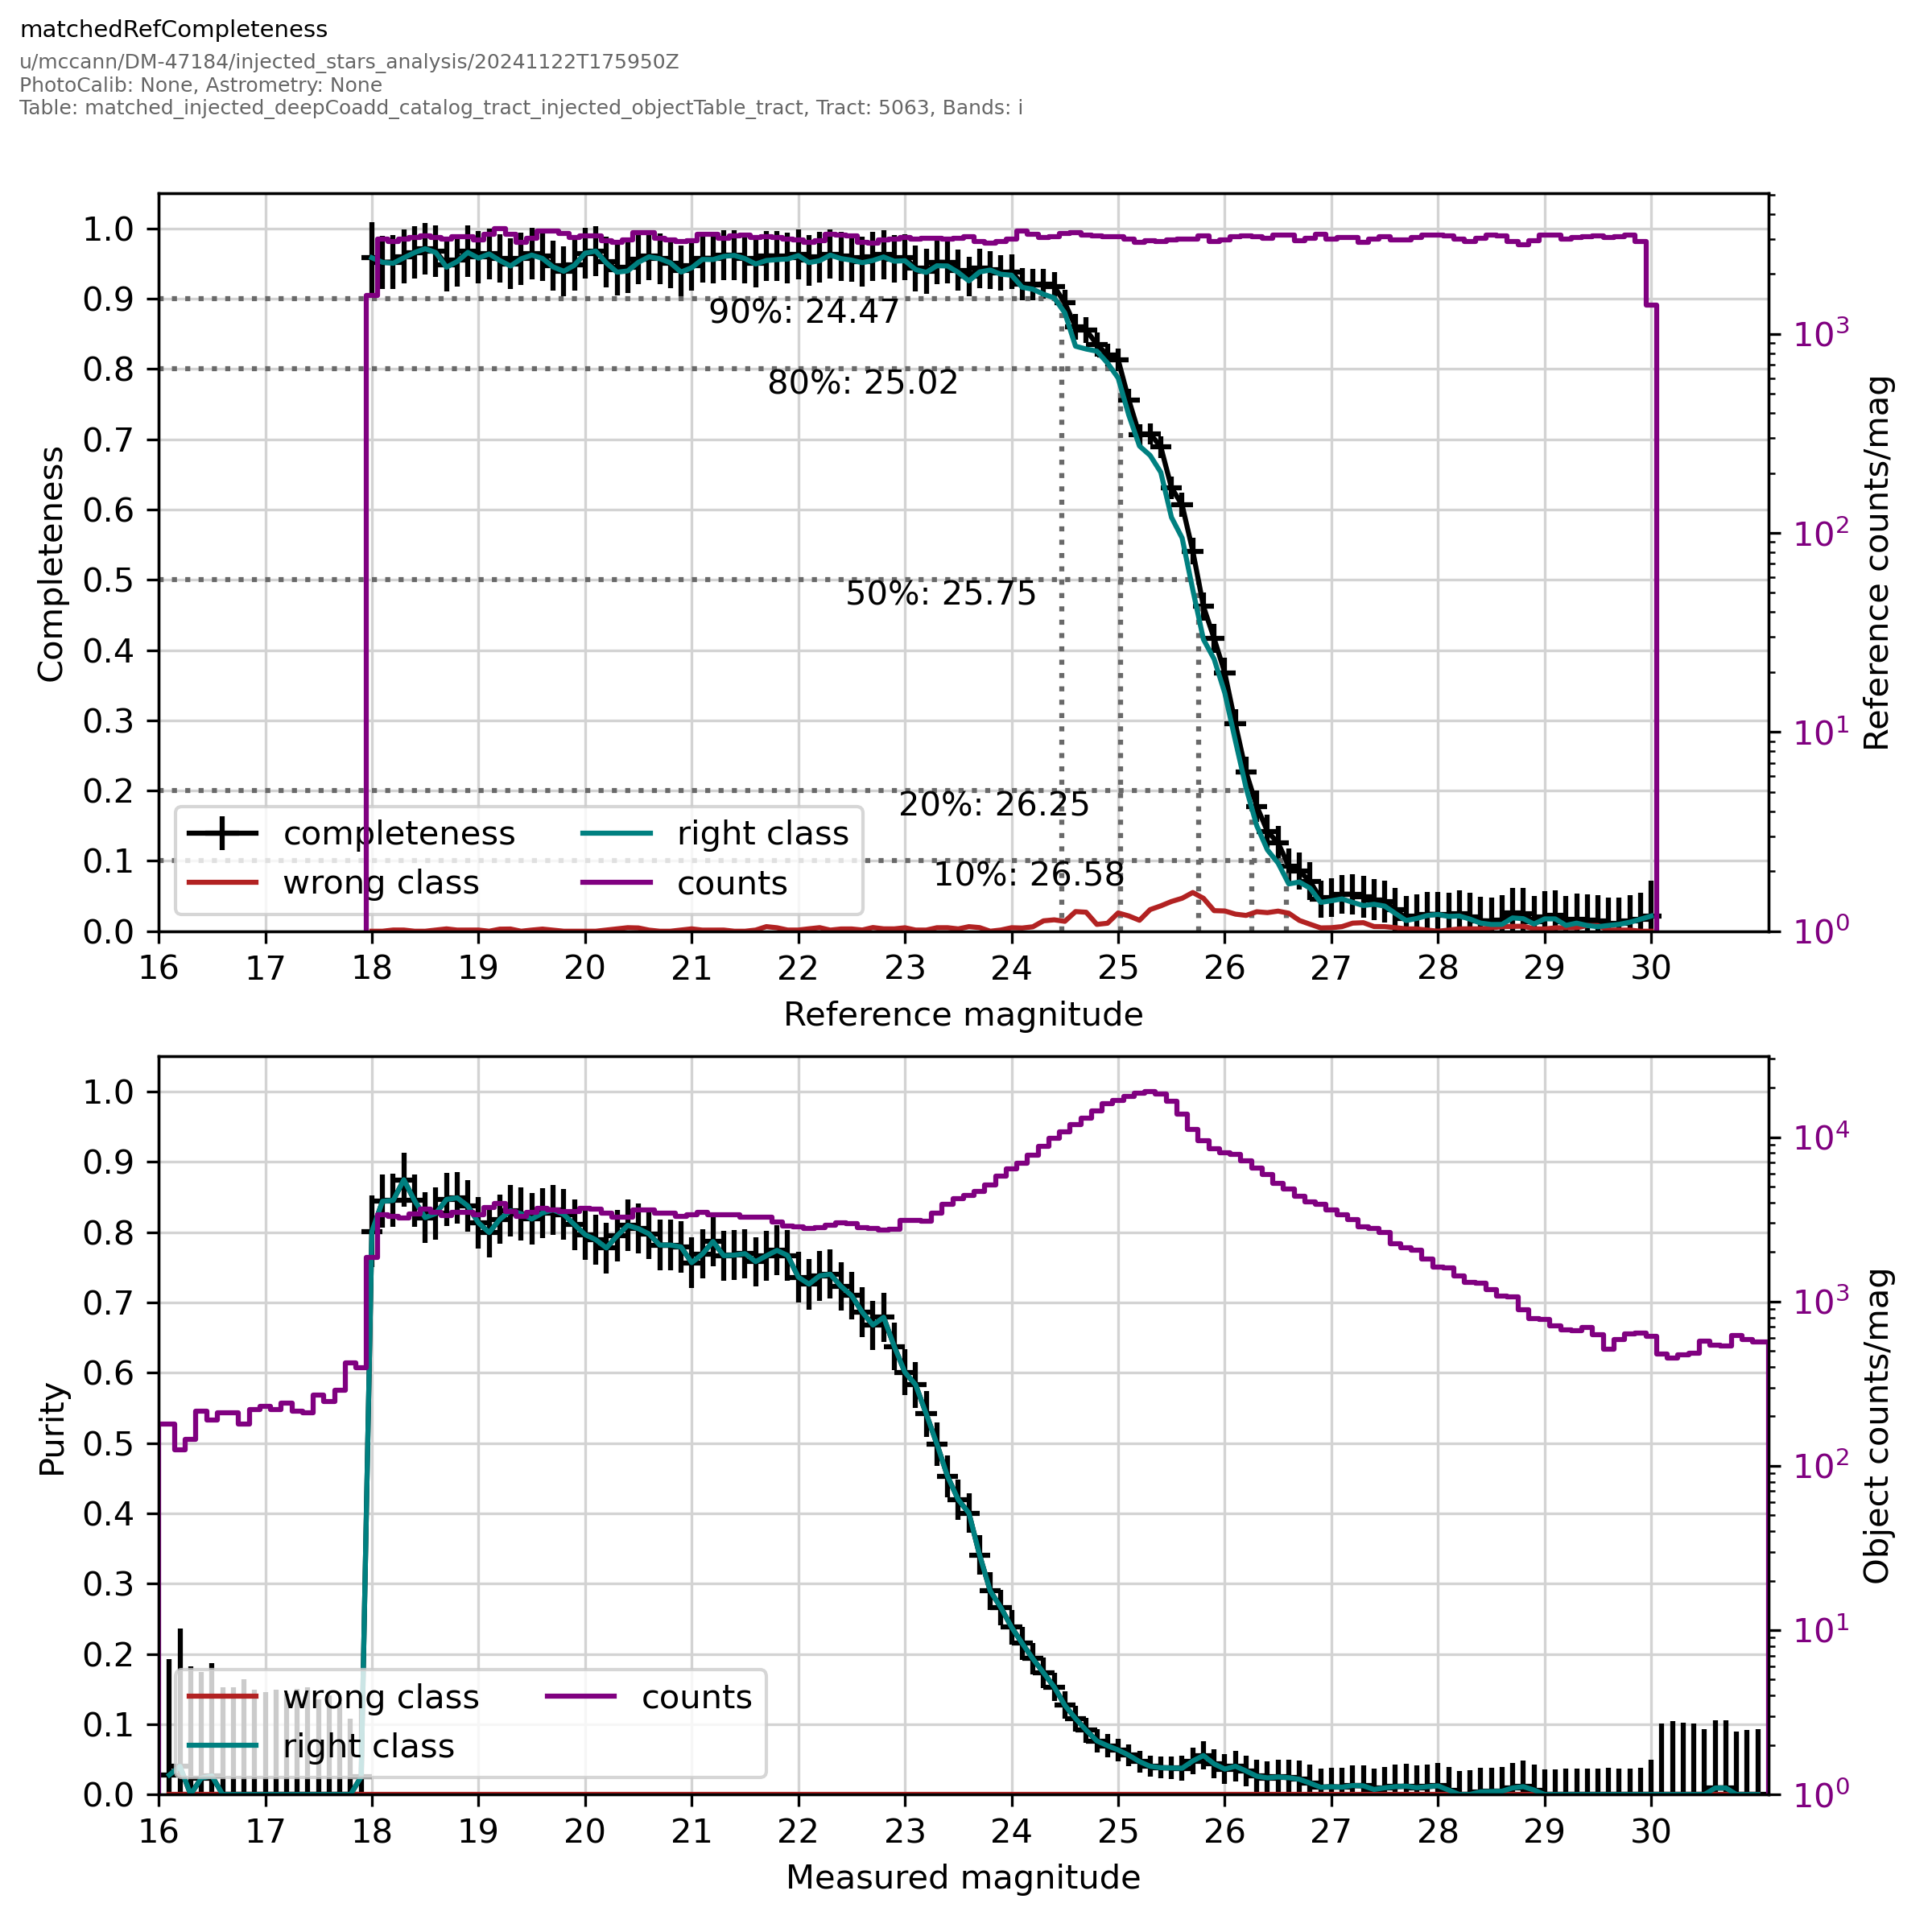
\includegraphics[width=0.75\textwidth]{sample_production_figures/matched_ref_completness_ssi_i.png}
    \caption{SSI based measurements of completeness and purity in the i-band.}
    \label{fig:ssi_comp}
\end{figure}

We also confirmed a strategy to use twilight observations to verify the system can accurately observe bright stars (1 mag brighter than 15 saturation lim).